\chapter{Modeling of the Vehicle}\label{cha:ModelOfVehicle}

The prototype model contains software, hardware and mechanical components. Software and hardware components are easy to change and to model after how the rest of the system is made and shall run. The vehicle, which is a mechanical plant, is provided to this project and therefore not changeable. This means that requirements about how the system should react, described in \secref{sec:Vehicledescription}, apply only for elements of the system that are external to the plant. In this chapter, a model of the vehicle is made to describe the power transfer from both the motor's and servomotor's rotational energy to the movement of the vehicle. Once, this model is established, it is possible to measure its output and apply a control on it, see \chapref{cha:ControlOfTheVehicle}.


\begin{figure}[H]
	\centering
	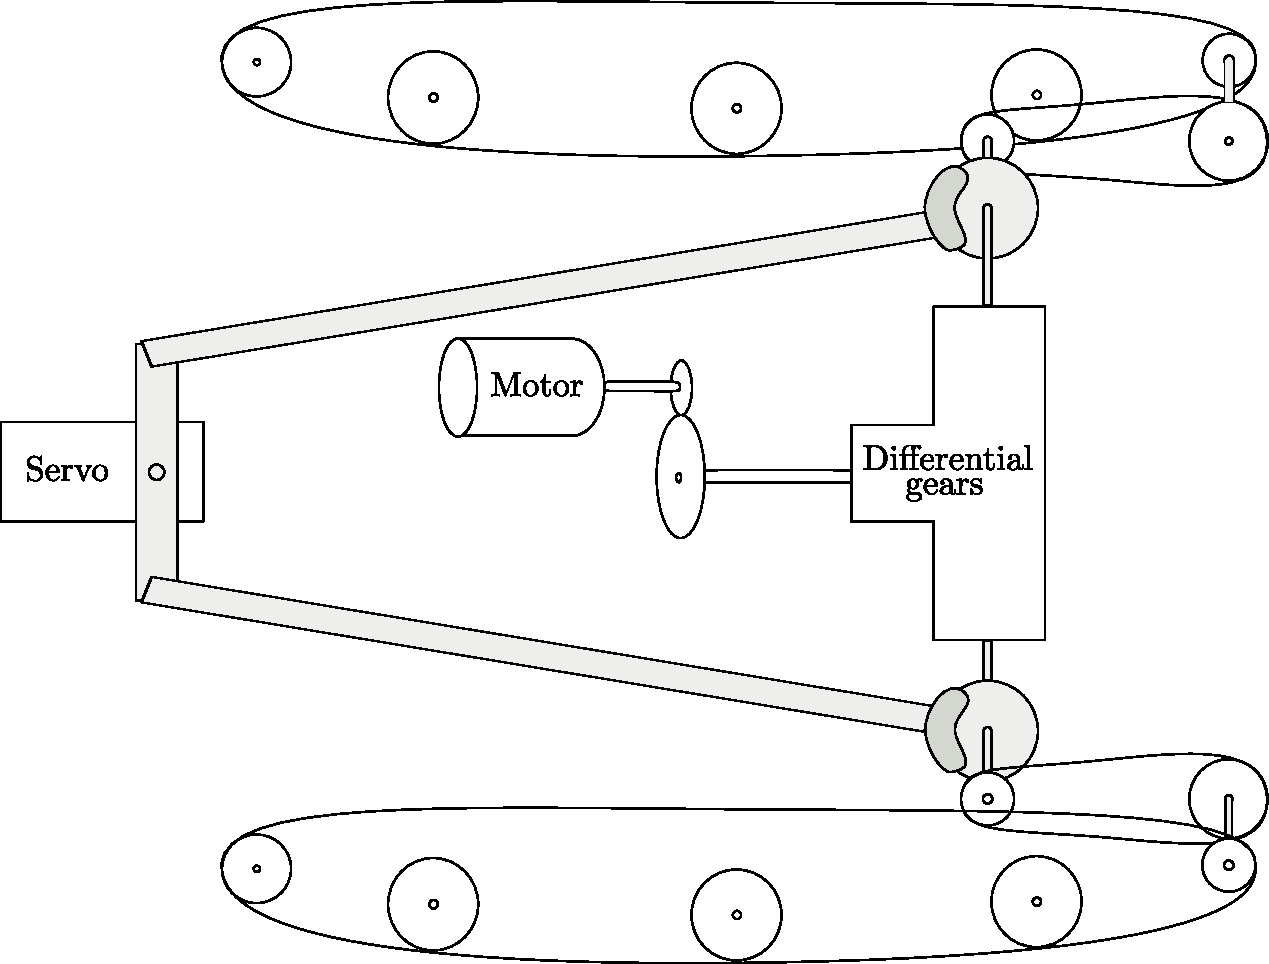
\includegraphics[width=\textwidth]{figures/completeMechanical.pdf}
	\caption{A mechanical diagram of the vehicle}
	\label{fig:completeMechanicalDiagram}
\end{figure}

The \figref{fig:completeMechanicalDiagram} shows both the drivetrain and steering mechanisms on the given vehicle. It is possible to identify and separate these two sub-systems. The parts that allows the vehicle to run includes the motor, the gears (that make the belts turn) and the belts themselves. On the other hand, the steering part includes the servomotor which acts on two shafts and is therefore capable of breaking one or the other belt, as stated in \secref{sec:Vehicledescription}. In the next sections, the motor and the drivetrain, which allow the vehicle to have a certain velocity, and the steering part, which allows the vehicle to turn, are modelled separately, and eventually recombined into a single model.